\documentclass{svproc}
\usepackage{geometry} % see geometry.pdf on how to lay out the page. There's lots.
\usepackage{hyperref}
\usepackage{graphicx}
\usepackage{gensymb}
\usepackage[affil-it]{authblk}
\usepackage[toc,page]{appendix}
\usepackage{pifont}
\usepackage{bm}
\usepackage{relsize}
%% \usepackage{draftwatermark}
\usepackage[mathscr]{eucal}
\usepackage{amsmath, amssymb, graphics, setspace}
%% \usepackage{amsart}
%% \usepackage{amsthm}
\usepackage[english]{babel}
\usepackage{listings}
\lstloadlanguages{Mathematica}
\usepackage{mathtools}
\usepackage{subcaption}
\DeclarePairedDelimiter{\norm}{\lVert}{\rVert}



\newcommand{\mathsym}[1]{{}}
\newcommand{\unicode}[1]{{}}

%% \newtheorem{exercise}{Exercise}
%% \newtheorem{theorem}{Theorem}
%% \newtheorem{corollary}{Corollary}
%% \newtheorem{lemma}{Lemma}
%% \newtheorem{conjecture}{Conjecture}
\newtheorem{observation}{Observation}

\newenvironment{sketch}{%
  \renewcommand{\proofname}{Proof Sketch}\proof}{\endproof}

\DeclareMathOperator{\atantwo}{atan2}
\DeclareMathOperator{\sign}{sign}
\DeclareMathOperator{\sense}{sense}

% \geometry{letter} % or letter or a5paper or ... etc
% \geometry{landscape} % rotated page geometry

% See the ``Article customise'' template for come common customisations

%%% BEGIN DOCUMENT
\begin{document}

\author{Robert L. Read\inst{1}}

\titlerunning{Calculating the Segmented Helix}
\title{Calculating the Segmented Helix Formed by Repetitions of Identical Subunits}

\institute{Public Invention, Austin, TX 78704, USA,\\
\email{read.robert@gmail.com},\\ WWW home page:
\texttt{https://www.pubinv.org}
}
\date{\today}


\maketitle

\abstract{
Eric Lord has observed:
\begin{quote}
  In nature, helical structures arise when identical structural subunits combine sequentially, the orientational and translational relation between each unit
  and its predecessor remaining constant.\cite{lord2002helical}
\end{quote}
If a robot is compsoed of modular structural subunits can change their shape, the shape of the robot
can change. If they all change in the same way, the robot will be a segmented helix of varying length.
Constant-time algorithms consistenting of analytic expressions are given for
the segmented helix generated from the intrinsic properties of a stacked object and its
conjoining rule.
The construction of these from the intrinsic properties of the rule for conjoining repeated subunits of arbitrary shape is provided,
allowing the complete parameters describing the unique
segmented helix generated by arbitrary stackings to be easily calculated.
Free-libre open-source interactive software and a website\cite{segmentedhelixmathfile} is provided which performs this computation
for arbitrary prisms along with interactive 3D visualization\cite{segmentedhelixinteractive}.
This allows the deduction of intrinsic properties of a repeated subunit from known properties of a segmented helix, as a chemist might
want to do.
Because the algorithms are efficient, a repeated subunit can be designed to create a segmented helix of
desired properties,
as a mechanical engineer or roboticist might want.
A theorem, proved in \cite{readfullsegmentedhelix} is provided that any subunit
can produce a toroid-like helix or a maximally-extended helix, forming a continuous spectrum based
on joint-face normal twist.
As a verification and demonstration, the software, website and paper compute, render, and
catalog an exhaustive ``zoo'' of 28 uniquely-shaped platonic helices,
such as Boerdijk-Coxeter tetrahelix and various
species of helices formed from dodecahedra.
}

\keywords{Helix, Variable Geometry Truss, Segmented Helix, Solid Geometry, Screw Theory, Platonic Helix}


\makeatletter
\newcommand{\subjclass}[1]{%
    \small
    \textbf{Mathematics Subject Classification:} #1}


\makeatother

\subjclass{ 97G40, 52B12}

\section{Introduction}

During the Public Invention Mathathon of 2018\cite{read2019mathathon}, software was
created to view chains of regular tetrahedra joined face-to-face.
The participants noticed whenever the rules
defining the face to which to add the next
tetrahedron
to were periodic, the resulting
structure was always like a discrete helix.

Although unknown at that time, this is a consequence of:
\begin{observation}[Lord's Observation]
  “In nature, helical structures arise when identical structural subunits combine sequentially, the orientational and translational relation between each unit and its predecessor remaining constant.”\cite{lord2002helical}
  \label{obs:lords}
\end{observation}
Although fairly obvious in hindsight from screw theory, we have found no articulation of this statement
in writing, so feel justified in naming it after the author of its earliest statement.
The surprising fact that DNA is a double helix allows replication and RNA synthesis by the unzipping and rezipping
of the helix.
However, the fact that it is helical in nature is unsurprising, since it follows directly from Observation\ref{obs:lords} and the
fact that the strands DNA are formed of repeated chemical units of approximately the same shape arranged sequentially.

The purpose of this paper is to provide mathematical
tools and software for studying arbitrary
segmented helices generated in this way. A proof of Lord's Observation is provided in a longer version \cite{readfullsegmentedhelix}.

Finding the properties of a segmented helix from three contiguous segments on the helix from screw theory\cite{wittenburg2016kinematics,kahn1989defining},
is explained and formulated.
An interactive, 3D rendering website written in JavaScript which allows both calculation and
interactive play and study is provided\cite{segmentedhelixinteractive}
(see Figure \ref{fig:dodecahedron}). This allows
a structure, or ``molecule'', coincident to a segmented helix to be designed
by adjustments to the repeated object, or for the shape of
a repeated subunit to be inferred from the intrinsic properties of the
segmented helix.
Kahn's method of helix fitting\cite{kahn1989defining,enkhbayar2008helfit,lee2007qhelix} is modified to cover some degenerate situations.

We exploit Lord's Observation to discover symmetry which allows us to compute the helix when subunits are joined face-to-face with
the same {\em twist.} Kahn was investigating proteins, which do not have faces, but geometric solids and other macroscopic solid objects do.
This concept can be generalized to a {\em joint face angle}, even if the
objects conjoined do not technically have flat faces.
This symmetry allows us to compute the parameters of the segmented helix purely from
properties intrinsic to a single object and the joining rule.
We prove that varying the {\em twist} of the joint faces through a complete rotation produces a smoothly varying
spectrum of shapes that always includes a torus-like shape and a
{\em zig-zag} planar segmented helix of maximal extent.
A robot thus constructed of identical modules, such as the TetRobot of \ref{fig:tetrahelices} which can change their shape allows the helix to coil and uncoil
predictably based on the math herein.


\begin{figure}
  \centering

  \subcaptionbox{Tetrahelix\label{fig:helixnodes}}
{\includegraphics[width=0.48\textwidth]{figures/UnifiedDrawing.png}}
\subcaptionbox{The 7-tet Public Invention Tetrobot\label{fig:tetrobot}}
{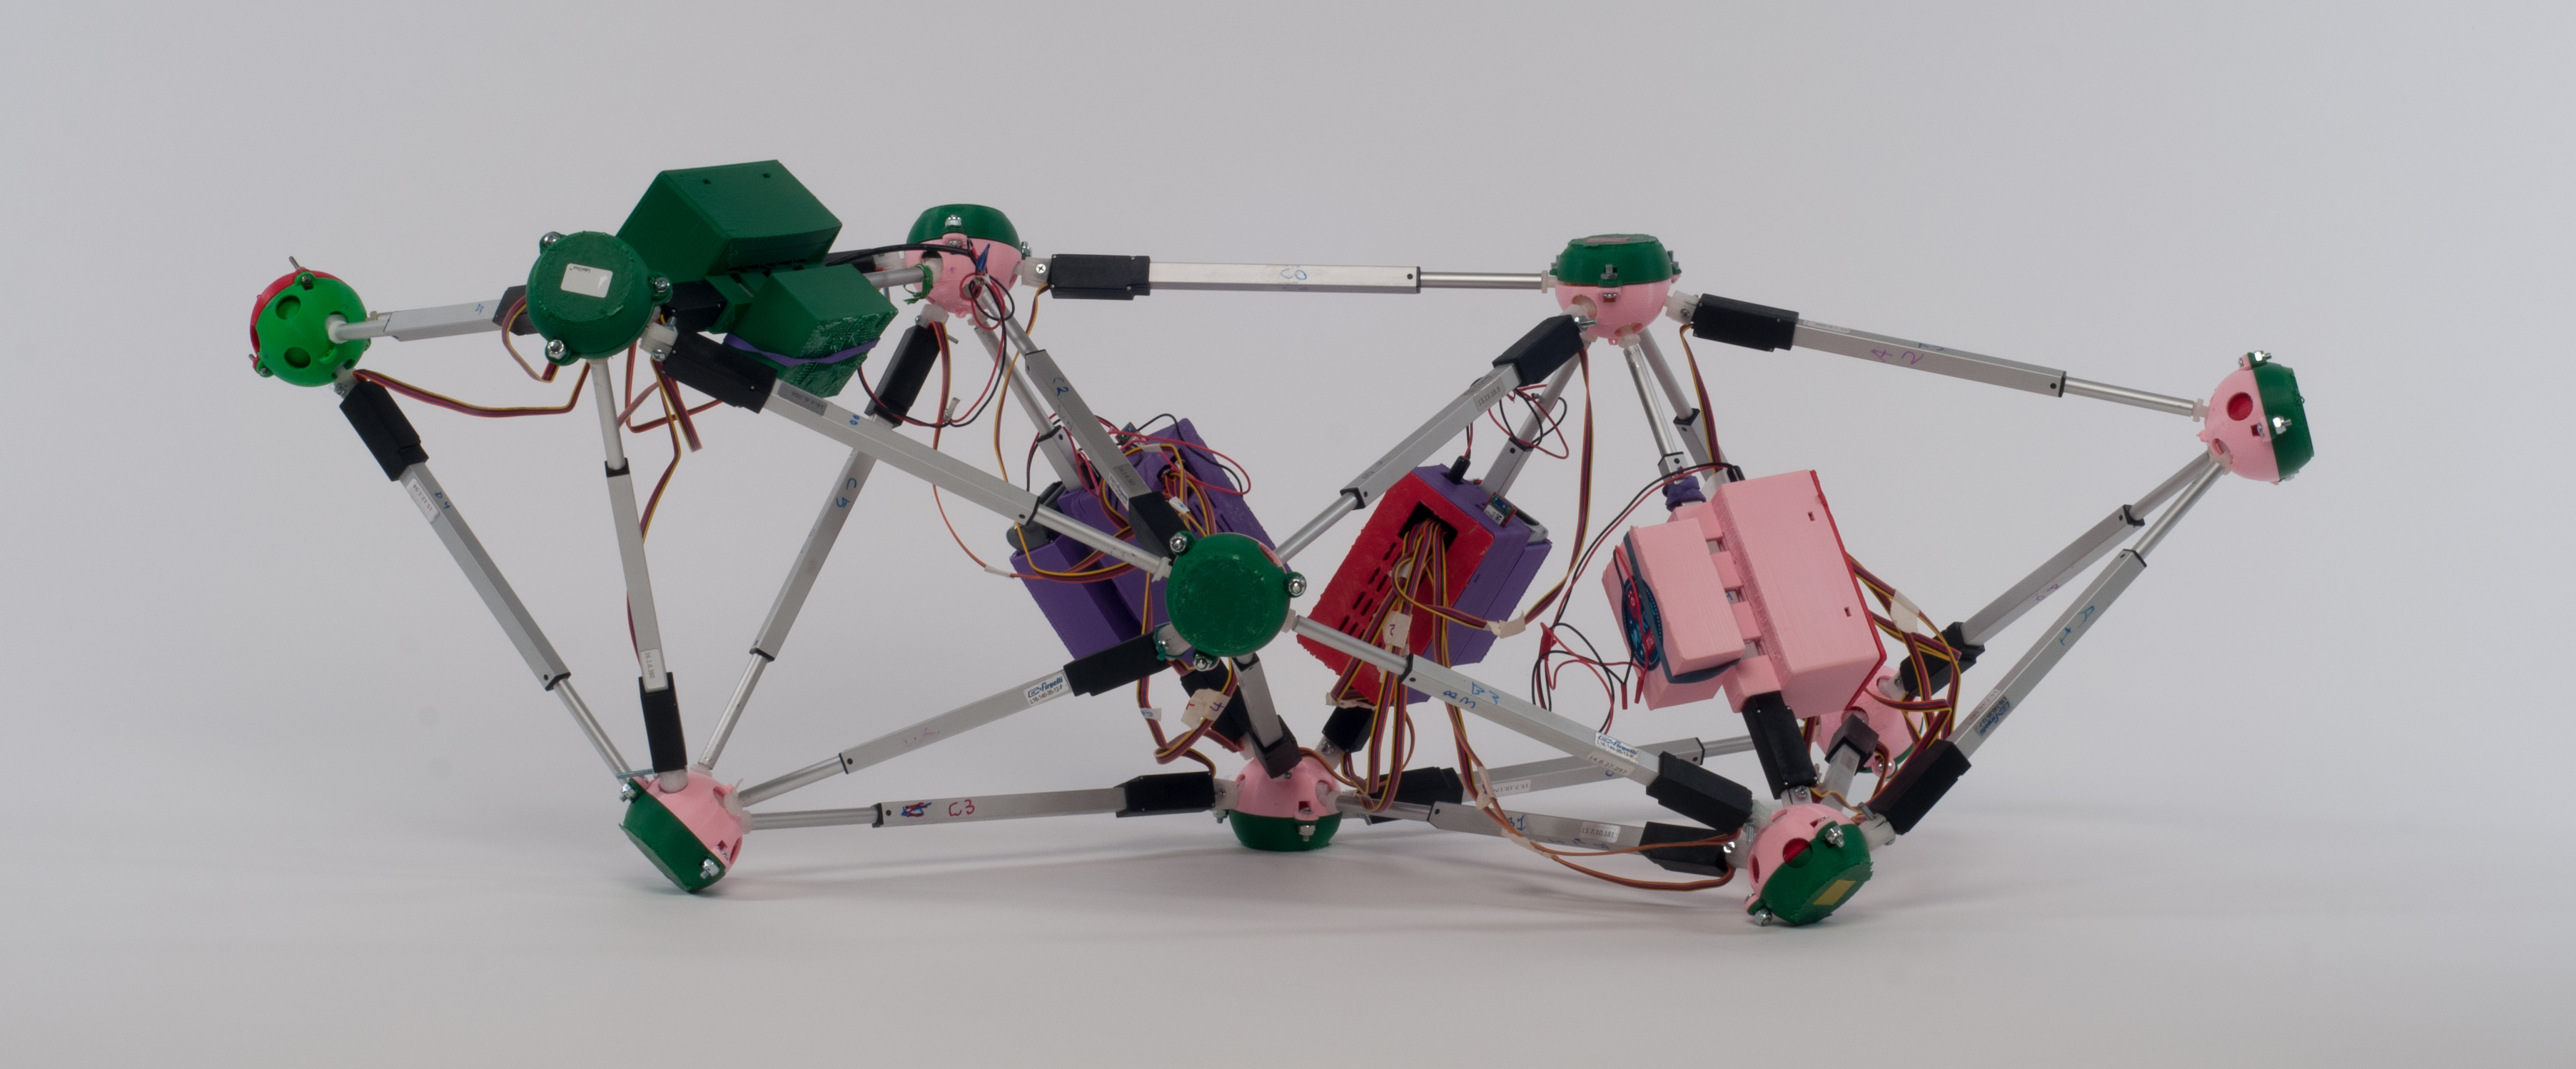
\includegraphics[width=0.48\textwidth]{figures/MedCantedCropped.png}}
\caption{Tetrahelix Robots}\label{fig:tetrahelices}
\end{figure}

\begin{figure}
     \centering
     \includegraphics[width=0.30\textwidth]{figures/Dodecahedral.png}
     \caption{Example Segmented Helix Generated From the Dodecahedron}
  \label{fig:dodecahedron}
\end{figure}

\section{The Segmented Helix}

A goal is to derive
the parameters for a continuous helix from such discrete objects by studying
a helix evaluated at integral points. Call such an object a {\em segmented helix}.
A segmented helix may be thought of as function that, given an integer, gives back a point in
3-space.
\begin{align}
    P_x(n) &= r \sin{n \theta}  \\
    P_y(n) &= r \cos{n \theta} \\
   P_z(n) &= n d
\end{align}

$d$ is the distance or {\em travel} along the helix axis between adjacent joints. In this canonical representation the helix axis is
the $z$-axis.
$\theta$ is the rotation around the $z$-axis
between adjacent points.
$r$ is the radius of the segmented helix.
Note that if $\theta = \pi$, a third form of degeneracy (to the human eye) occurs:
that of a segmented helix
which is a zig-zag contained completely within a single plane.

If one thinks of the segmented helix as describing a polyline in 3-space,
the properties of that polyline are of interest.
Considering only the {\em intrinsic} shape of the segmented helix that
are independent of position and orientation in space,
there are three degrees
of freedom: $r,d,$ and $\theta$.

\begin{figure}
     \centering
     \includegraphics[width=0.30\textwidth]{figures/ABCDFigure.png}
     \caption{Naming of measures}
  \label{fig:naming}
\end{figure}

Figure \ref{fig:naming} demonstrates naming convention concepts.
It is a screen shot taken from the interactive website\cite{segmentedhelixinteractive}.
The software allows parallax by supporting interactive rotation,
which makes the 3D structure easier to perceive;
please visit the interactive page during this discussion of naming conventions.

In Figure \ref{fig:naming} and the website, we represent the object as a prism
with triangular cross-section, because this is
the simplest physically realizable macroscopic object that supports a face-to-face connection.
In this diagram, the
points $A,B,C$, and $D$ are represented by the sphere of the same color as the label. The view is roughly in the direction of
the axis of the segmented helix, which is drawn as a dark green arrow, pointing in the positive $z$ and positive $x$ direction,
parallel to the $XZ$-plane.
For ease of viewing, the entire segmented helix has been raised by two units on the $y$ axis.
The segment $\overline{BC}$ has coordinate $y = 2$, is aligned with the $z$-axis, and centered in the $z$ direction.

The positive $x,y$ and $z$ axes are shown by the red, green, and blue axis arrows, respectively.
Following computer graphics convention, the $y$ axis is oriented vertically.
The points $A,B,C$, and $D$ correspond to $P(0), P(1), P(2)$, and $ P(3)$, respectively,
for a segmented helix aligned
to the raised axis (not the $z$-axis).
A thin green polyline represents the segmented helix, and thus connects the joints $A,B,C$, and $D$.
The points are wrapping around the axis clockwise, with an angle of $\theta = 56.6 \degree$ as
shown by the on-screen protractor as the rotation from one point to the next. As will be explained in Section \ref{sec:facenormal},
$\tau$ is the face-on-face joint rotation, in this case of $45 \degree$.
The helix angle $\phi = 39.7 \degree$ is rendered by a protractor on the $y = 0$ plane;
this is the angle between the axis
and of the helix and the $z$ axis, and therefore the angle of any one segment against the helix axis.

Any point on the segmented helix has a closest point on the axis of the helix.
In particular, the points closest to the
joints are called {\em joint axis points}.
Then $d$ is the distance along the axis between consecutive joint axis points.

A line is drawn from the blue point $B$ to a black sphere on the helix axis,
the joint axis point, denoted $B_a$. Analogously, $C_a$ is the point
on the axis closest to the green point $C$.


A segmented helix located in space is completely determined by
the parameters $r,d,\theta$,
a vector describing the axis
of the helix, and the position of any one joint.

Because the segmented helix is a discrete structure, one can reframe the concept of {\em pitch} as {\em sidedness $s$}:
how many segments (sides)
make a complete rotation?

The following concepts and conventional variable names for them will be related:
\begin{itemize}
\item $L$ is the distance between any two adjacent joints (between $B$ and $C$, for example).
  \item $r$ is the distance between a joint and the helix axis (between $B$ and $B_a$ for example).
  \item $\theta$ is the rotation about the helix axis between two consecutive joints.
  \item $c$ is the length of a chord formed by the projection of the segment between two points projected along the axis of the segmented helix (a chemist may recognize this as the distance between residues on a {\em helical wheel} projection).
  \item $d$ is the distance along the axis of the helix between any two joint axis points (between $B_a$ and $C_a$ in Figure \ref{fig:naming}, for example, rendered as a small black and blue
    sphere, respectively).
\item $\phi$ is the angle between any vector between two adjacent joints and the axis of the helix. In physical screws used in mechanical engineering, this is analogous to the {\em helix angle}.
  \item $p$ is the pitch of the helix, the distance traveled in one complete rotation.
  \item $s$ is the number of segments in a complete rotation (in general not rational).
\item  Finally, we find it useful to define the {\em tightness} of a segmented helix
as travel divided by radius, a number
analogous to the extension of a coil spring or slinky.
A torus-like segmented helix has zero tightness and a zig-zag has
maximum tightness. The letter $t$ represents tightness.

  \end{itemize}
These quantities are related:
\begin{align}
    c &= 2r\sin{\frac{\theta}{2}} \\
    L^2 &= c^2+d^2  \\
    \arctan{\frac{c}{d}}  &= \phi \\
    s &= \frac{2 \pi}{\theta} \\
    d &= L \cos{\phi} \\
    p &= d \cdot s \\
    t &= d / r
\end{align}

Please see the longer version of this paper for a full discussion
of some convenient conventions.
Sections \ref{sec:pointaxis} and \ref{sec:facenormal}
relate these properties to properties intrinsic to the joint or interface between
two segments or objects in the segmented helix.

\label{sec:SegmentedHelix}

\section{The Intrinsic Properties of Periodic Chains of Solids}

Although fairly obvious from Chasles' Theorem, in order to prove Observation \ref{obs:lords},
additional clarification is helpful.
If chains of identical repeated 3D units are conjoined identically, they are {\em periodic chains},
and they generate a segmented helix coincident on their joints.
Identical objects conjoined via a rule
produce periodic chains of objects that are uniformly intersected
by segmented helices and may be degenerate in one of
three ways that might not strike the human eye as a helix at first glance:
\begin{enumerate}
\item The segments may form a straight line.
\item The segments may be planar about a center, forming a polygon or ring.
\item The segments may form a planar saw-tooth or zig-zag pattern of indefinite extent.
\end{enumerate}

There are two complementary ways of learning about such segmented helices.
In one approach, we may have knowledge of the segmented helix and
wish to learn about the subunits and the rule with which the subunits are combined.
In the other approach, one may know {\it a priori} exactly the
relevant properties of the objects and the rule with which they combine
and seek to compactly describe the segmented helix they create.

\section{Periodic Chains Produce Segmented Helices}

A periodic chain is, in fact, a simple object which demonstrates tremendous symmetry.
Before using this symmetry in the construction of the segmented helix corresponding to a periodic chain,
it is valuable to
prove that such a segmented helix indeed exists for every periodic chain.
Because periodic chains are merely a clarification of the ``identical structural subunits''
of Observation \ref{obs:lords},
this theorem proves that observation.

\begin{theorem}[Segmented Helix]
  \label{thm:helix}
  Consider $N$ identical objects which each have two points, $A$ and $B$, called {\em joints}. Call
  $\overrightarrow{AB}$ the {\em axis} of this object.
  Consider the frame of reference for this object to have
  its axis on the $z$-axis with $B$ in the positive direction, the
  midpoint of the object being at the origin.

  Consider any rule that conjoins $A$ of object $i+1$ to $B$ such that
  from the frame of reference of $i$, the object $i+1$ and anything rigidly
  attached to it is always in the same position in the frame of reference for $i$.
  Informally, $i+1$ ``looks the same'' to $i$, no matter what $i$ is chosen, $i < N$.
  Call a chain of $N$ identical rigid objects conjoined via a rule that
  conjoins $A_{i+1}$ to $B_i$ in such a way that every vector
  of $B$ is always in the same position relative to a frame of reference
  constructed from $A$, a {\em periodic chain.}

  Any periodic chain of three or more objects has a unique segmented helix
  whose segments correspond
  to the axes of these objects.
\end{theorem}

A proof is provided in the longer version of this paper\cite{readfullsegmentedhelix}.

Consider
objects which are, taken as individuals, highly asymmetric.
For example,
the $B$ face does not have to be the same size as the $A$ face. In fact,
the object itself might be shaped like the letter ``C'', and not completely
enclose the axis. Taking the idea further, the object might be spiky
like a stellated polyhedron or a sea urchin, and still be joined by
joints relatively close to the center of the object. (This paper does not
address the issue of self-collision of the objects,
which would have to be considered if attempting to make a period chain
of sea urchins).

It is perhaps not obvious that building a chain of such objects
produces a segmented helix, and therefore that the helix angle is the
same for each object, but this is a corollary of Theorem \ref{thm:helix}.

\section{{\em PointAxis}: Computing Segmented Helices from Joints}
\label{sec:pointaxis}

Kahn\cite{kahn1989defining} has given a method for computing
the axis of a helix in the context of chemistry.
This method uses the observation that the angle bisectors
of the segments on a segmented helix are perpendicular to
and intersect the axis of the helix.
Because chemical helices may not be perfect and because the measurement of positions may not be perfectly accurate,
it is common for chemists to use regression and fitting methods to fit helix parameters to observed positions
on the helix.
Kahn's method was a prelude to some error-tolerant methods applicable to
the realm of organic chemistry\cite{enkhbayar2008helfit}.
This paper is concerned only with pure geometry. Also, Kahn was writing in 1989,
and more convenient computing tools are now available.
The algorithm presented, called {\em PointAxis}, here can be considered a modification of Kahn's algorithm,
which relies on the ability, working in the realm of pure geometry, to position the segments on the axes
to simplify the derivation and computation.

\subsection{A Sketch of the 4-Point Method}

Using tools from linear algebra and well-documented algorithms, a sketch of finding the segmented helix from
four consecutive known points $A,B,C$, and $D$ is:
\begin{itemize}
\item Construct a rigid transformation that places the points conveniently on the $z$-axis and balanced
  around the $y$-axis.
\item Compute the bisectors of the angle between object axes $ \angle{ABC}$, called $\overrightarrow{B_b}$ and the
  bisecting angle $\overrightarrow{C_b}$ of $\angle{BCD}$.
  If the points are collinear, they are a special case.
\item Because these angle bisectors point at the axis of the segmented helix, their cross product is a vector
  in the direction of the axis. If $\overrightarrow{B_b}$ and $\overrightarrow{C_b}$ are parallel or anti-parallel the cross product is not defined
  and we have special cases.
\item  Otherwise the vectors $\overrightarrow{B_b}$ and $\overrightarrow{C_b}$ are skew, and the algorithm for the closest points on
  two skew lines provides two axis points $B_a$ and $C_a$ on these vectors which
  are the closest points on those lines and are also points on the helix axis.
\item The distance between $B_a$ and $B$ is the radius, and the distance between $B_a$ and $C_a$ is the travel $d$ along the axis.
  \item The angle between $\overrightarrow{B - B_a}$ and $\overrightarrow{C - C_a}$ is $\theta$.
\end{itemize}

\subsection{Rotating into Balance from Face Normal Vectors}

\label{sec:balance}

In order to use the {\em PointAxis} algorithm, we need a way
to compute points $A$ and $D$ in balance around the axis $BC$.

\begin{figure}
     \centering
     \includegraphics[width=0.80\textwidth]{figures/Balance.png}
     \caption{A Balanced Configuration}
  \label{fig:balancediagram}
\end{figure}


Figure \ref{fig:balancediagram} shows a downward view of a
balanced configuration (though raised above the origin
instead of at the origin).
$A$ (the red sphere) is a reflection of $D$ (the purple sphere) across
the $y$-axis.
Both $A$ and $D$ are hanging downward.
If the structure were hung on a point at the origin, it would
be physically balanced.
As shown in the following, it is always possible to achieve this balance,
even though a single object
itself is not symmetric; in this figure the normal of the $B$ face is not symmetric with $C$ face.

That this is always possible is important enough, if only for
the convenience of calculation, that we consider it a Lemma:
\begin{lemma}[Balance Lemma]
  For any segmented helix with selected consecutive joints $A,B,C$ and $D$,
  there is a rigid transformation which positions it such that:
  \begin{itemize}
  \item The segment $BC$ is centered on the $z$-axis:
    $(B_x = 0 \wedge B_y = 0 \wedge C_x = 0 \wedge C_y = 0)
    \wedge B_z < 0 \wedge C_z = -B_z$.
  \item The joints $A$ and $D$ are in rotational balance about
    the $y$ axis, as if they were weights hanging downward:
    $A_y = D_y \wedge A_y \leq 0 $ and
    $A_x = -D_x \wedge A_z = -D_z$.
  \end{itemize}
  \label{lem:balance}
\end{lemma}

A proof sketch is provided in the longer version of this paper\cite{readfullsegmentedhelix}.

The screw axis may now
be computed from either the four points $A,B,C$, and $D$ or from the transformation
matrix created to balance them.

\subsection{The 4-Point Method}

Four consecutive points completely determine at least one segmented helix.
Consider
only the helix that makes the least rotation between these points,
though more rapidly rotating helices will also intersect these points.
The {\em PointAxis} algorithm
takes four such points. Without loss of generality $B$ and $C$
are assumed to be centered on the $z$-axis, and that a
rotation has been performed to balance $A$ and $D$ so that $A_x = -D_x, A_z = -D_z$, and $A_y = D_y$. Thus the input to
{\em PointAxis} in fact has only three degrees of freedom, which determine the three intrinsic properties $r,d,\theta$
which completely define the shape of a segmented helix (but not its location in space).


In the derivations below, we rely on certain facts about
the segmented helix formed by the stack of objects, the first
of which is key:
\begin{itemize}
\item By virtue of Lemma \ref{lem:balance}, without loss of generality, think of any member whose faces
  and twist generate a non-degenerate helix as being ``above'' the
  axis of the helix. Furthermore choose to place the object in
  this figure so that $B_y = C_y$, that is, that the members are symmetric
  about the $z$-axis.
  $A$ and $D$ are ``balanced'' across the $YZ$-plane,
  and $A_x = -D_x$ and $A_y = D_y$.
\item Every joint ($A,B,C$, and $D$) is the same distance $r$ from the axis $H$ of the helix.
\item Every member is in the same angular relation $\phi$ to the axis of the helix.
\item Since every member of a non-degenerate helix cuts across a cylinder around the axis,
  the midpoint of every member is the same distance from the axis
  which is, in general, a little a less than $r$. In particular the midpoint $M$
  whose closest point on the helix axis $m$ is on the $y$-axis and
  $\| \overrightarrow{M_m} \| < \| \overrightarrow{B_b} \|$.
\item The points ($A_a,B_a,C_a,D_a$) on the axis closest to the joints ($A,B,C,D$)
  are equidistant about the axis and centered about the $y$-axis. In
  particular, $\| \overrightarrow{B - B_a} \| = \| \overrightarrow{C - C_a} \|$.
\end{itemize}

From the observations that $\| \overrightarrow{B - B_a} \| = \| \overrightarrow{C - C_a} \|$
it becomes clear that the helix axis is in a plane
parallel to the $XZ$-plane, it intersects the $y$-axis, but in general is
not parallel to the $z$-axis.

Because the angle bisectors of each joint are in general skew, and intersect the
axis perpendicularly, the algorithm
for the closest points on two skew lines finds $B_a$ and $B_c$.

However, a segmented helix has
tremendous symmetry, and the angle bisectors are very far from being two
generally skew lines. In fact, by taking advantage of the fact that the
generating rule for an object chain requires similarity in every joint,
the objects can be arranged as in Figures \ref{fig:naming} and \ref{fig:threemembersdiagram}.

{\em PointAxis} takes a length and a point $D$ known to be in
a specific relation to $B$ and $C$.

This careful arrangement of the axes
allows the computation of $\phi$, the angle between the helical axis
and the $z$ axis. This, in combination with symmetry and the knowledge
that the helical axis is in the $XZ$ plane, supports computing the
points on the axis corresponding to the joints directly from $\phi$.

This algorithm coded below is simple enough that Mathematica\cite{Mathematica} can
actually produce a symbolic closed-form formula for all computed valued
in terms of $L, x, y$, and $z$.
However, these formulae are less comprehensible to the
human eye than this algorithm.
Their existence does open
the possibility that, for example, the derivative representing
the change in $r$ with a change in $D$ could be calculated.

\subsection{Degenerate Cases}

Define the angle bisector vectors:
\begin{align}
  \overrightarrow{B_b} &= B - (A + C)/2 \\
  \overrightarrow{C_b} &= C - (B + D)/2
  \end{align}
The fundamental insight that the axis of the helix $H$ can be
computed by a cross product of the angle bisector
vectors ($\overrightarrow{B_b}$ and $\overrightarrow{C_b}$) applies only
when the angle-bisectors have a non-zero length and when
they are not anti-parallel. When they are of zero length, this is
the degenerate case of a straight line coinciding with all segments.
When $\overrightarrow{B_b}$ and $\overrightarrow{C_b}$ are parallel and pointing in opposite directions,
the zig-zag degeneracy occurs.
The math for both of these cases is provided in the longer paper\cite{readfullsegmentedhelix}.

\subsection{Standard Case}

However, the most general case is simpler and can be worked
out with standard linear algebra operations. In the math below,
which is a direct analog of our coded solution, the tremendous symmetry of the ``balance'' condition
permits the computation to proceed with
using mostly scalar operations. There is some hope that
this would allow closed-form expressions to be produced, perhaps
with the aid of a symbolic computation system such as
Mathematica\cite{Mathematica}. If completed, this would
allow us to give closed-form solution to the intrinsic properties
of all the 28 Platonic helices enumerated in Sec \ref{sec:platonic}.

Once $\overrightarrow{H}$ has been calculated, the signed travel along the axis $d$ is
the scalar projection of a segment $\overrightarrow{C - B}$ onto $\overrightarrow{H}$.
From this $\phi$ is directly calculable. $\phi$ allows
a direct calculation of the $x,y$ and $z$ components of the
point $B_a$ on the axis pointed to by $\overrightarrow{B_b}$.
$r$ is the distance between $B_a$ and $B$. $c$ and $\theta$
are easily computed from these values.

\begin{align}
  \overrightarrow{H} &=  \begin{bmatrix} -2 B_{b[y]} B_{b[z]} \\ 0 \\ 2 B_{b[y]} B_{b[x]}  \end{bmatrix} \\
  d &= \frac{L B_{b[x]}}{\sqrt{B_{b[x]}^2 + B_{b[z]}^2}}  \\
  \phi &= \atantwo{(H_z,H_x)} - \pi/2  \\
  c &= \sqrt{L^2 - d^2}
\end{align}

In this approach to calculation, it is easiest
to compute the axis point $B_a$ corresponding to $B$ and
use it to complete our computations.

From trigonometry and utilizing the facts that
\begin{align}
\phi &= \arccos{(d/L)} \\
\sin{(\arccos{x})} &= \sqrt{1 - x^2}
\end{align}
  it
can be shown that
the $x$ and $z$ component of $B_a$ are:
\begin{align}
  B_{a[x]} &= \frac{d\sqrt{1 - (d/L)^2}}{2} \\
  B_{a[z]} &= -\frac{d^2}{2L}
\end{align}

However, this computation exposes another special case: when the
helix angle $\phi$ is $\pi /2$, the segmented helix is
torus-like. In this case the axis point $B_a$ is in fact
on the $y$-axis, and so only $B_{a[y]}$ is need:
\begin{align}
  B_{a[y]} &=  \frac{L B_{b[y]}}{2 B_{b[z]}}
\end{align}
Except for in the toroidal case,  $B_{b[x]}$ must be taken into
account, but it is non-zero, so we can divide by it.
By imagining a plane pressed downward from the
object axis to the helix axis, it is apparent that $B_{a[y]}$
is proportional to a ratio of the angle bisector
$B_{b[y]}/B_{b[x]}$ times the $B_{a[x]}$ value:
\begin{align}
  B_{a[y]} &=  \frac{ B_{b[y]} B_{a[x]}}{ B_{b[x]}}
\end{align}

Having computed all of $B_a$, the remaining intrinsic properties are easily
calculated:

\begin{align}
  r &= \norm{B - B_a}  \\
  \theta &= 2 \arcsin{\frac{c}{2r}}
\end{align}

\subsection{Comparison to Screw Theory}

The full version of this paper\cite{readfullsegmentedhelix} provides an exposition of how to compute the same parameters
using screw theory. The interactive software computes the parameters using both methods and compares the results as a test.
Although roughly equivalent, the method given here is more direct.
Modern
computer algebra systems such as Mathematica\cite{Mathematica} it might be possible to use these ``algorithms'' to produce closed-form
expressions of closed-form (algebraic) inputs. For example, the Platonic solids all have lengths and face normals which
can be specified exactly in closed (though irrational) form.
Thus in the future it might be possible to produce a closed-form expression for the
radius of one of the Platonic Dodecahelices of unit edge length, which would be harder to do from screw theory.
Because this section has given analytical expressions, it is reasonable to compute the derivative of these
parameters in terms of changes to basic module shape analytically. This would allow a robot made of modules
to conform to a desired shape, such as maximum extent or maximum coiling, with a single change made
to each module.

\section{The Joint Face Normal Method}
\label{sec:facenormal}

{\em PointAxis} takes a point $A$ known to be in a specific, balanced relation
to $B, C$ and $D$. A chemist might know four such points from crystallography
and be able to move them into this symmetric position along the $z$-axis.

However, one might instead know something of the subunits and
how they are conjoined, without actually knowing where points $A$
and $D$ are.

Take as given these intrinsic properties of an object, and additionally the
rule for how objects are laid face-to-face. That is, knowing the length between two
joint points and a vector normal to the faces of the two joints, we almost have
enough to determine the unique stacking of objects. The final piece
needed is
the {\em twist}. When face $A$ of a second objects is placed on face $B$
of a first object so that they are flush (that is, their normals are in opposite directions),
it remains the case that the second object can be rotated about the normals. To
define the joining rule, attach an {\em up vector} to each object, or more appropriately
since we are dealing with a helix, an {\em out vector} that points away from the axis.
Then a joining
rule is ``place the second object against the first, joint point coincident to joint point,
and twist it so that its out vector differs by $\tau$ degrees from the out vector of the first
object.'' In this definition, the out vectors are considered to be measured against the plane
containing the two axes meeting in a joint.

Define the {\em joint plane} to be the plane which contains the two faces meeting in a joint.
Define the {\em joint line} to be the line through the joint perpendicular to the joint plane.
Define the {\em joint angle} to be the angle of the first axis to the second measured about
the joint line.
The twist $\tau$ is the change in the a vector attached to the object rotated about the joint
line by the joint angle. That is, take any vector attached to the first object, place it at
the joint, rotate it about the joint line via the joint angle. $\tau$ is the difference
between the angle of this vector measured against the joint plane and the angle of the
out vector of the second object measured against the joint plane.

If the objects are macroscopic objects which have faces, this is the same as the rotation
of the axis of the second object relative to the first in the plane of the coincident faces.
Define intrinsic properties:

\begin{itemize}
\item Given an object with two identified faces, labeled $B$ and $C$, assume there are normalized
  vectors $\overrightarrow{N_B}$ and $\overrightarrow{N_C}$
  from each of these points that are aligned with the axis of the conjoined object attached to
  that face. These normals might be enforced by the fact that flat faces are joined in the joint plane.
  However, molecules don't have faces; this conjoining relationship may be enforced some other way.
\item The length $L$ of an object, measured from joint point $A$ to joint point $B$.
\item A joint twist $\tau$ defining the change in computed out-vector between objects,
  measured at the joint face.
\end{itemize}


For computer programmers with a graphics library supporting transformation matrices such
as THREE.js\cite{dirksen2013learning},
it is relatively easy to code the math to adjoin objects
face-to-face based on the face normals, simulating the physical act of
matching flat faces between macroscopic objects.


\section{Changing $\tau$ Smoothly Changes Tightness}

Upon implementing our interactive ability to vary $\tau$, the following
theorem becomes visually apparent.

\begin{theorem}[Twist Spectrum]
  For any choice of non-parallel face normals having non-zero $x$ or $y$ components,
  changing the twist angle $\tau$ through a complete rotation ($0 \leq \tau \leq 2\pi$)
  smoothly varies the segmented helix
  between a torus and flat cases.
\end{theorem}

A proof is provided in the full version of this paper\cite{readfullsegmentedhelix}.
The Twist Spectrum theorem asserts that if the twist between the modules of a robot
can be varied consistently, then the robot can easily move through a toroid-like shape
into a linear shape and back. If it does not self-collide, it can even change the chirality
or handedness of the helix it forms.

In the calculator page
the $\tau$ that produces the minimum tightness (torus-like) and maximum tightness (zig-zag) to the
nearest 360-degree is numerically calculated,
with the labels {\em Minimum Tightness $\tau$} and {\em Maximum Tightness $\tau$}.

When the joint face normals are coplanar vectors, then the minimum tightness $\tau$ is
always $0$, and the maximum tightness occurs when $\tau = \pm \pi$.
These values deviate from $0$ and $\pi$ roughly in proportion
to the non-coplanarity of the normals.

Varying $\tau$ smoothly varies the tightness of the coiling of the helix,
moving through very linear cases towards a torus,
to a torus, to a very linear case on the other side.

In fact it is possible that there is always a ``tightest coil''
which does not self-intersect. If we had many objects,
they could be packed into a convenient space by computing the $\tau$
of the tightest non-self-intersecting coil and stacking them this way.
If $\tau$ can be changed, perhaps via motors in a robot arm,
the object stack smoothly telescopes and contracts forming a
linear actuator.
A repeated molecular subunit that changed shape in
response to an external magnetic or electric field or chemicals in the surrounding
environment would be a telescoping nanomachine or nanoactuator.
\begin{figure}
  \centering

  \subcaptionbox{$\tau = -3.75 \degree$ }
{\includegraphics[width=0.32\textwidth]{figures/coiling/tau-375.png}}
\subcaptionbox{$\tau = 0 \degree$}
{\includegraphics[width=0.32\textwidth]{figures/coiling/tau0.png}}
\subcaptionbox{$\tau = 3.75 \degree$}
{\includegraphics[width=0.32\textwidth]{figures/coiling/tau375.png}}
  \subcaptionbox{$\tau = 7.5 \degree$ }
{\includegraphics[width=0.32\textwidth]{figures/coiling/tau75.png}}
  \subcaptionbox{$\tau = 15 \degree$ }
{\includegraphics[width=0.32\textwidth]{figures/coiling/tau15.png}}
\subcaptionbox{$\tau = 30 \degree$}
{\includegraphics[width=0.32\textwidth]{figures/coiling/tau30.png}}
\subcaptionbox{$\tau = 60 \degree$}
{\includegraphics[width=0.32\textwidth]{figures/coiling/tau60.png}}
\subcaptionbox{$\tau = 120 \degree$}
{\includegraphics[width=0.32\textwidth]{figures/coiling/tau120.png}}
\subcaptionbox{$\tau = 180 \degree$}
{\includegraphics[width=0.32\textwidth]{figures/coiling/tau180.png}}
\caption{Coiling via change to $\tau$}\label{fig:coiling}
\end{figure}

\subsection{Implications}

One of the implications of having an easily-calculable understanding of the math
is that it may be possible to design helices
of any radius and pitch by designing periodic (possibly irregular) objects.
Combined with slight
irregularities, this means there exists a basis to design molecular helices
out of ``atoms'' which correspond to our objects.

A modular robot constructed out of repetitions of the same
shape-changing module will always
produce a helix
whose precise shape can be controlled by uniformly changing the shape of all
of the modules. Such a robot might change its shape radically from a toroid
to a linear extension.

\section{Applying to The Boerdijk-Coxeter Tetrahelix}


%% TODO: Join this figure with the other.




The {\em tetrobot}\cite{sanderson1996modular,HamlinSandersonCMS,lee1999dynamics,TetrobotBook,} is the concept of completely
modular robot built entirely out of tetrahedra whose side lengths can
be varied under electronic control. Such robots tend to be inherently
tensegrities\cite{mirletz2014,NTRT,paul2006}, although where the cable lengths
have shrunk to zero.
The current work was instigated by the author's research with seven-tet tetrobot
\ref{fig:tetrobot}.
In particular, it is possible to construct a tentacle or snake-like or
variable-geometry truss configuration of tetrahedra which, in its relaxed
mode, is a regular tetrahelix.

The Boerdijk-Coxeter tetrahelix (BC helix) (see Figure \ref{fig:helixnodes}) is a periodic chain of conjoined regular tetrahedra
which has been much studied\cite{coxeter1985simplicial,sadler2019periodic,fuller1982synergetics,read2018transforming}
and happens to have irrational measures, making it an ideal
test case for these algorithms. Because the face-normals can be calculated and the
positions of the elements of the BC helix directly calculated, we can use
it to test the algorithms, and in fact these algorithms give the same rotation.



However, it should be cautioned that the helix which Coxeter identified\cite{coxeter1985simplicial}
goes through every node of every tetrahedron. Constructing the helix going
through only ``rail'' nodes allows irregular tetrahelices to be designed\cite{read2018transforming}
(see Figure \ref{fig:helixnodes}).
However, the segmented helices defined in this paper do neither; rather, it is most natural to
imagine them moving through the centroid of a face of a tetrahedron.
This is a segmented helix of
very small radius ($0.0943$) compared to the other two approaches
($\frac{3\sqrt{3}}{10} \approx 0.5196$) which measure the radius to the
vertex of the tetrahedron, but it has
the advantage that it is far more general. For example, it is
clearly defined if one used truncated tetrahedra.
The rotation of a
segment matches the BC helix analytical solution
($\theta = \arctan{-3/2} \approx 131.810$),
because a screw transformation does not depend on selecting a point for the radius.



\subsection{Confirming Periodic Twists}

The Boerdijk-Coxeter tetrahelix has an irrational rotation about the angle,
meaning that is aperiodic.
There is no number of perfectly regular tetrahedra that can be joined to get back to exactly
the same position.
A recent paper by Sadler, Fang, Clawon and Irwin\cite{sadler2019periodic} has explored this
and given an explicit formula for a {\em twist} exactly as defined in this
paper in order to produce a periodic tetrahelix. The explain how to compute a twist
that gives a period of, for example, seven tetrahedra ($\approx 80.43 \degree$). It is gratifying that this angle does
in fact produce a period-7 tetrahelix as shown in Figure \ref{fig:periodseven} produced from
the interactive software described herein.

In order to demonstrate the utility of the calculations explained in this paper,
periodic chains of the five regular Platonic solids joined face-to-face so that their vertices coincide,
which form {\em Platonic helices}, are explored.
Such tetrahelices, icosahelices, octahelices and dodecahelices
have been mentioned in a number of papers\cite{elgersma2016quadrahelix,babiker2012combinatorial,lord2001sphere}, but not exhaustively studied in
the purely helical form.
Because in some cases Platonic segmented helices may be found in nature or
related to structures found in nature\cite{lord2004gamma,pearce1990structure},
our longer paper\cite{readfullsegmentedhelix} has calculated all such platonic helices (there are 28 unique ones) and given
their parameters in a table, the first such description of this ``zoo'' of structures.


\section{Acknowledgements}

Thanks to Prof. Eric Lord for his direct communication.
The enthusiasm of the participants of the 2018 Public Invention Mathathon
initiated this work.

\bibliographystyle{unsrt}
\bibliography{shelix}

\appendix


\end{document}
